%%%%%%%%%%%%%%%%%%%%%%%%%%%%%%%%%%%%%%%%%%%%%%%%%%%%%%%%%%%%%%%%%%%%%%%%%%%%%%%
%
% Implementation of the application
% 
%%%%%%%%%%%%%%%%%%%%%%%%%%%%%%%%%%%%%%%%%%%%%%%%%%%%%%%%%%%%%%%%%%%%%%%%%%%%%%%
\chapter{Implementation of the application}
\label{cha5}

The application is structured by different packages. Each of them providing a specific benefit to the program as a whole. Before speaking about those modules, we will talk about the actual requirements of the application. After that, each module will be explained in detail. % After that, the last section will deal with problems and possible solutions.

\section{Requirements definition}
\label{sec5.1}

Focus of this application is the possibility to automatically process forms and retrieve the data of the forms. Hence the application should be able to deal with several files and process them. But, since there is a big variety of forms and every company have different structures, retrieving all necessary information can fail. If this happens, a user has to review scanned documents that contain errors. If it doesn't fail, the data should be stored without the need of a review.

We visualized these requirements as an UML use case diagramm in figure \ref{totalApplicationCase}.

\begin{figure}[ht!]
\centering
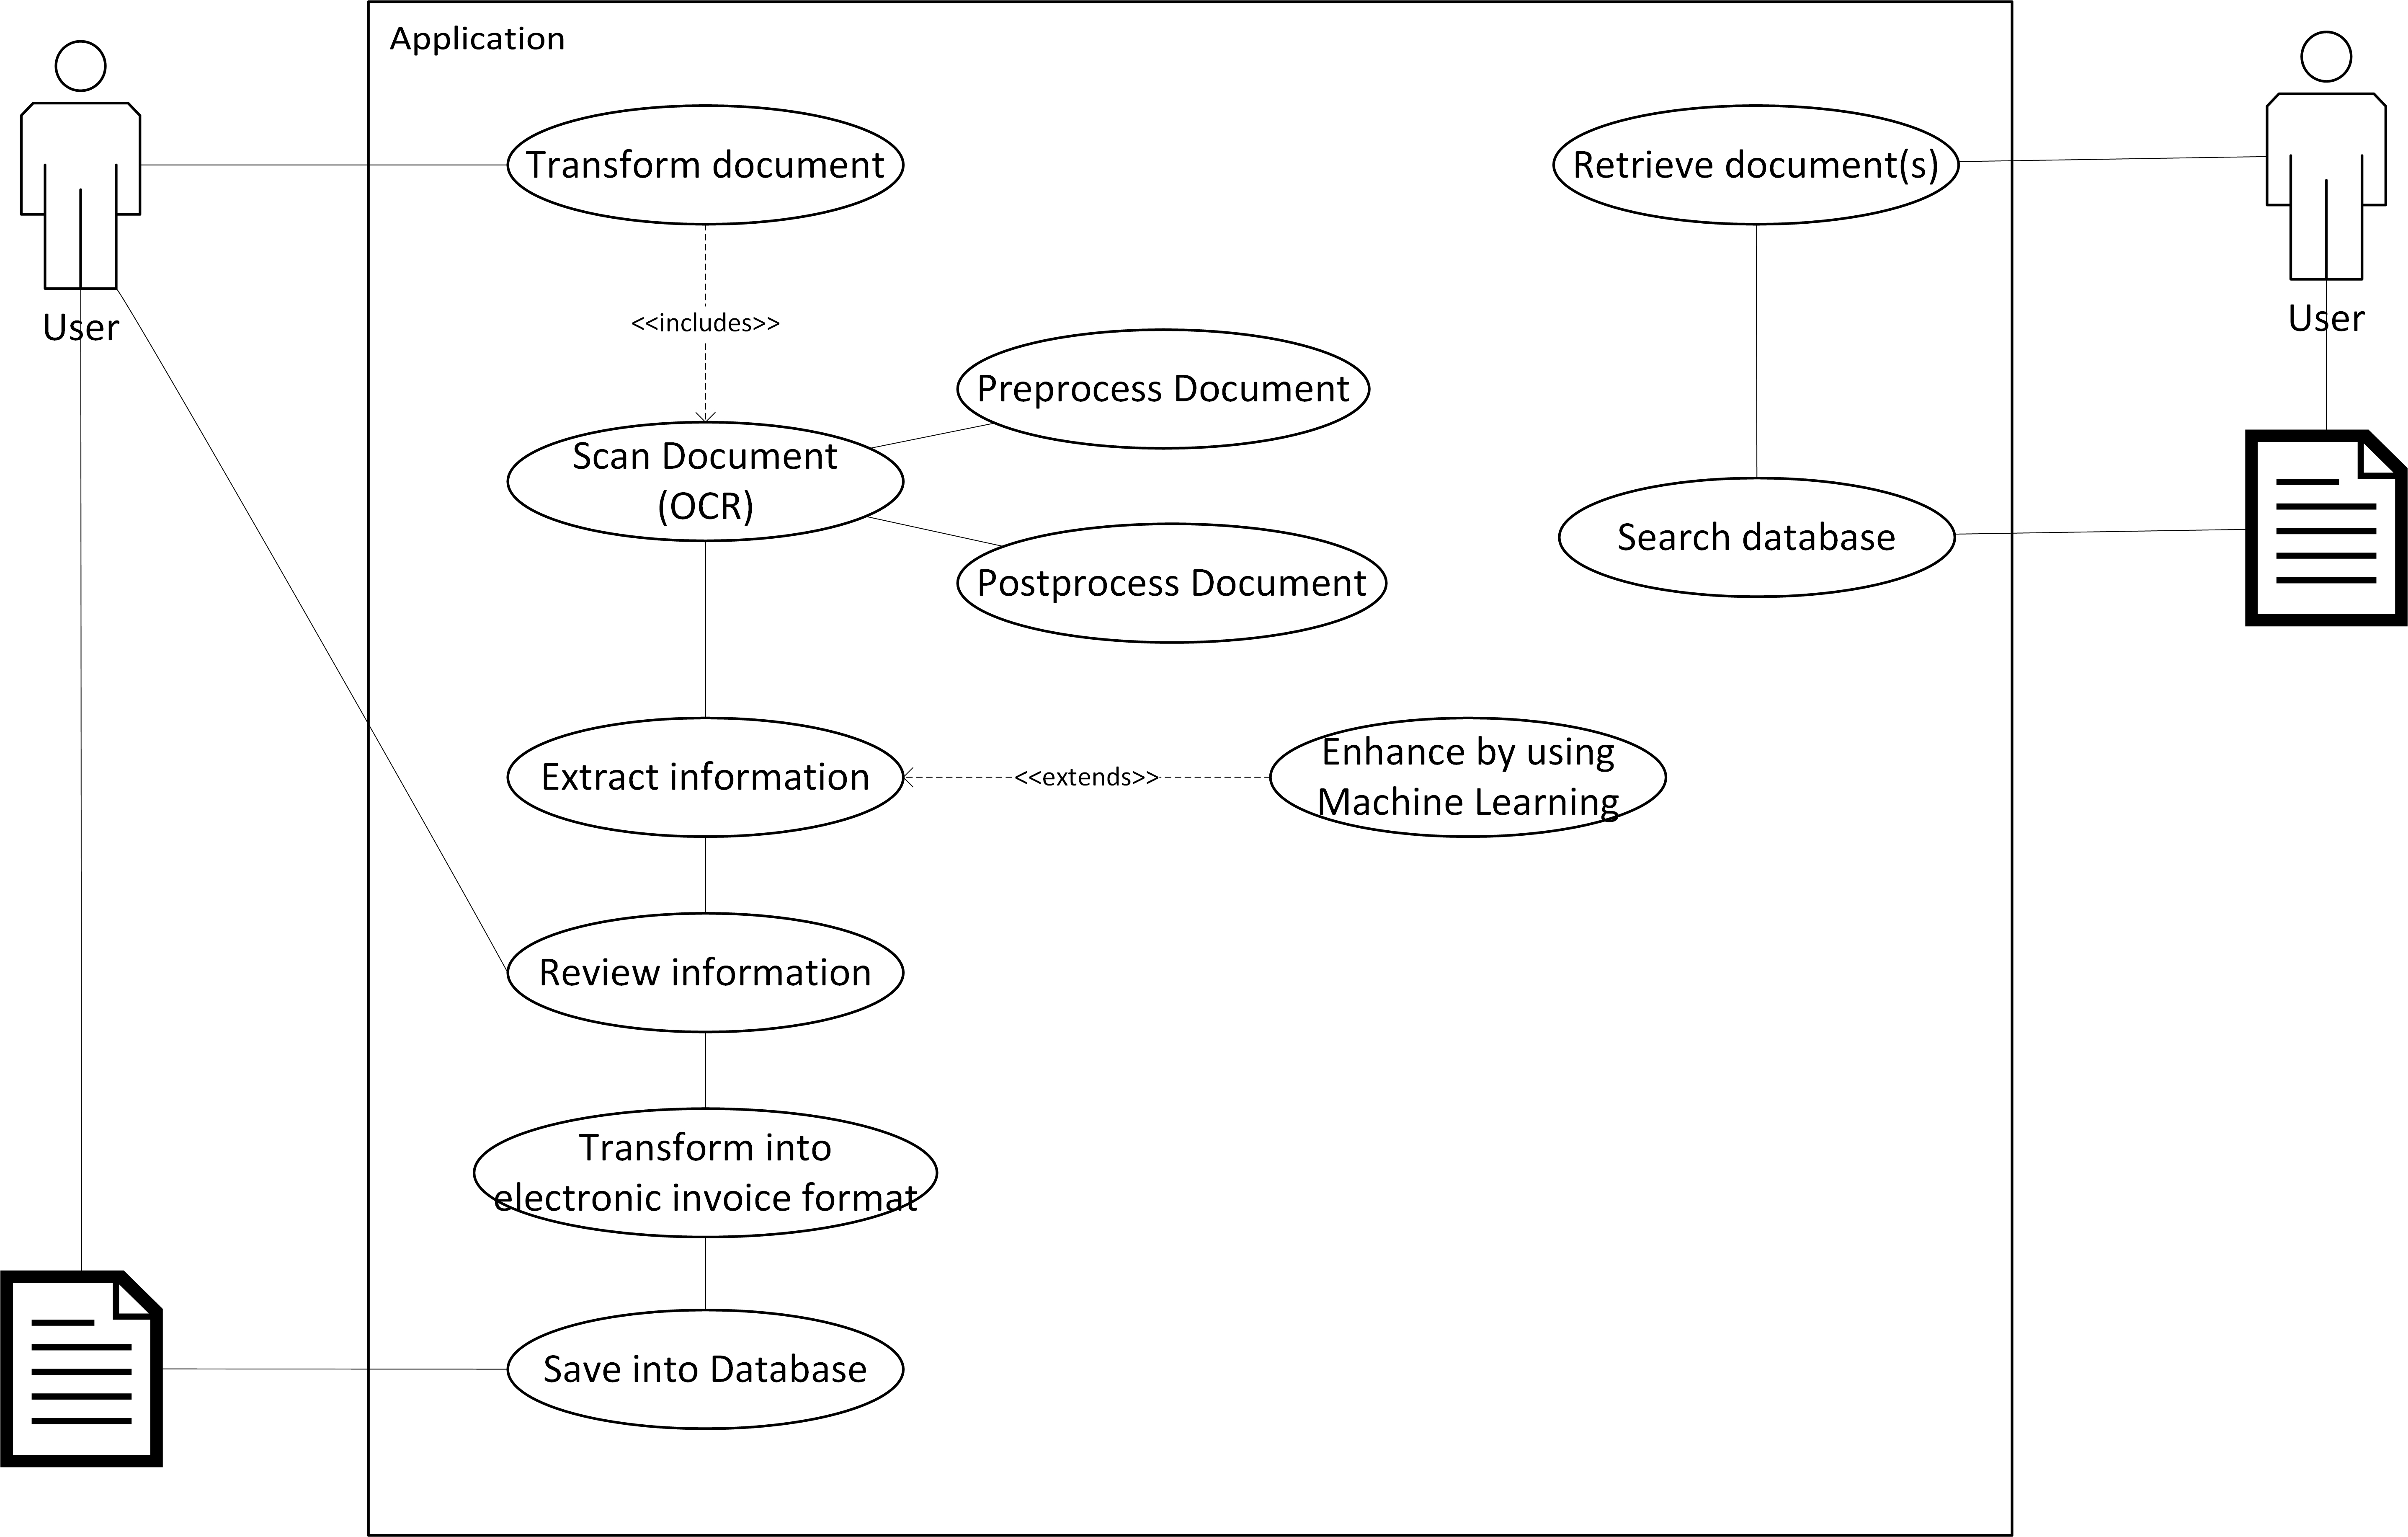
\includegraphics[width=\textwidth]{Images/UseCase/TotalApplicationCase.jpg}
\caption{Use case of the application \label{totalApplicationCase}}
\end{figure}

To improve the process of gathering data, a machine learning approach should be implemented that facilitates retrieving data and to speed-up form processing over time.

Output of the application should be a storage of the processed forms, appended with electronic invoice information that is valid against the basic- or comfort-level of the ZugfErd-Invoice standard.

\section{Definition of modules}
\label{sec5.2}

Following the Separation of Concerns principle (SoC) we want to separate all logical parts of the application into different modules.
What the application will do is to take an invoice, read it (1), extract the information out of it (2), improve the information by using machine learning techniques (3) and eventually convert it to the ZugFerd-format (4). All these processes should be manageable for the user using a GUI (5).
Hence, we will define five different modules:
\begin{enumerate}
	\item \emph{OCR}: After the user has passed an document to the application, this module will process the document and read it using OCR techniques. Therefore, this module will be named \emph{OCR}.
	\item \emph{Extraction}: This module will deal with the business logic regarding the retrieval of information from the processed document. Therefore, it will also give input and get output from the third module.
	\item \emph{ML}: In this module we will implement methods to improve future information extraction.
	\item \emph{Transformation}: Eventually, the extracted information and the processed document will be transformed into a new electronic invoice that is conform with the ZUGfERD-format.
	\item \emph{GUI}: In order to facilitate the process of entering and retrieving invoices, another module will be used that deals with all sorts of user interaction. As this application will have an graphical user interface, we will call this module \emph{GUI}.
\end{enumerate}

\section{Architectural concept}
\label{sec5.3}

The application is structured by different packages that each contribute to the application as a whole.
As shown in figure \ref{applicationUML}, there are 7 different packages. 

\begin{figure}[ht!]
\centering
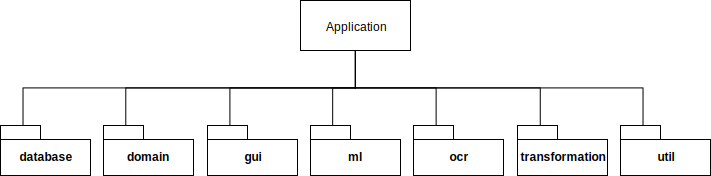
\includegraphics[width=\textwidth]{Images/UML/ApplicationUML.png}
\caption{Packages of the application \label{applicationUML}}
\end{figure}

In section \ref{sec5.2} we have already defined most of the packages before. However, we want to explain the other packages as well. While the modules OCR, ML, Transformation and GUI are present, the module Extraction is missing. The reason for that is that the actual extraction of information is a domain specific part of our application. Hence it can be found in the domain package. Figure \ref{domainUML} shows a detailed view of the domain package. This package again is structured by the subpackages 'bo', 'dao', 'helper' and 'service'.

\begin{figure}[ht!]
\centering
%\def\svgwidth{\columnwidth}
%\includesvg{Images/UML/DomainUML}
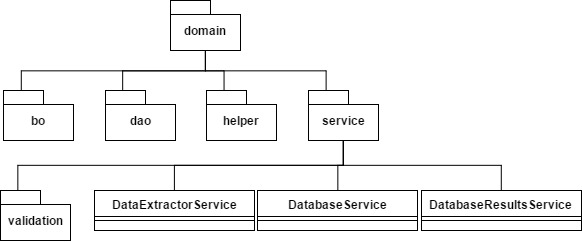
\includegraphics[width=\textwidth]{Images/UML/DomainML.png}
\caption{The domain package in detail \label{domainUML}}
\end{figure}

'Service' contains the DataExtractorService class which is responsible for the actual extraction of invoice information. To do this, several other classes are called, some of them located in other packages (e.g. the utils package).

Besides the DataExtractorService class, there are other important classes. The ZugFerdExtendService class adds the valid ZugFerd invoice to the pdf document. The DatabaseService is responsible for saving the reviewed invoice documents (as the last part of the use case in \ref{totalApplicationCase}). When a user searches for invoice documents, the DatabaseResultsService is called that performs the actual request.

In addition to those classes, the package validation also contains classes to validate not only the mandatory invoice information, but also the accounting records.

The application will make use of an architectural design pattern, the Model-View-Controller (MVC) pattern.
This pattern separates the application in three parts: The model, that contains the data of a domain, the view, which presents the given data in a specific way to the user, and the controller, that is responsible for the communication between the other two. Figure \ref{MVCpattern} visualizes this behaviour.

\begin{figure}[ht!]
\centering
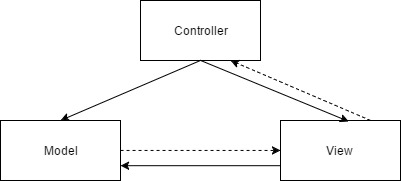
\includegraphics[width=100mm]{Images/UML/MVC.png}
\caption{The Model-View-Controller pattern \label{MVCpattern}}
\end{figure}

Using this architectural pattern, we are more flexible and can easily change views or models since these are only loosely coupled. Hence the graphical user interface will be steered by a controller which retrieves data from the database and shows it to the user using the javaFX framework and .fxml-Files (those represent the 'View' in the MVC pattern). Input and changes the user makes in the view will be transported by the controller to the model which is stored in the database again.

To access the database we will use classes for each business object. The package BO contains classes that represent a table. A data-access-object (DAO) will be used to retrieve data from the database. Note that these two packages are present in the domain package (see figure \ref{domainUML}).
This application will also make use of an object-relational mapping framework (Hibernate), which facilitates the conversation between table data and java objects.

\section{Module 1 - OCR}
\label{sec5.4}

The OCR module deals with the processing of the document. Therefore, we will use Googles Tesseract as described in chapter 3. In order to use it, we use Tess4J as a Java wrapper. TesseractWrapper.java is the class that initiates a tesseract instance. With initOcr() the tesseract instance is getting called. It returns a String as result. 

We set HOCR to true, which means that our output will not only be a String containing the processed words, but in a structured way. HOCR is a xml-structured document first proposed by \cite{Breuel07}. Using this output we are not only able to retrieve the processed words, but also their position in the document.

The package hocr contains necessary java classes to represent this document in an objective-oriented way. The string output of the TesseractWrapper class can be given to the constructor of the HocrDocument class, that completely parses the string and divides it into multiple HocrAreas, HocrParagraphs, HocrLines and HocrWords.
Before the actual step of processing the image, we want to improve its quality. Therefore, we use the ImagePreprocesser class. Any kind of document inserted will first converted to a BufferedImage. Then preprocess() can be called which executes multiple algorithms on the image:

\begin{lstlisting}[caption={Image preprocessing}]
public BufferedImage preprocess() {
    try {
        ...
        BufferedImage outputFile = this.resizeImage(image);
		...
        outputFile = this.adjustDPI(image);
		...
        outputFile = this.deSkewImage(image);
		...
        outputFile = this.greyScaleImage(image);
		...
        outputFile = this.deSpeckleImage(image);
		...
        return outputFile;
        } 
  	...
}
\end{lstlisting}

Most of those calculations are made using ImageMagick, a powerful open source library with several useful commands to apply on images. It is licensed under the Apache 2.0 license. In order to use it inside our application we are using IM4Java which is cited by ImageMagick itself\footnote{the citation can be found here: https://www.imagemagick.org/script/develop.php, last visited on 06.03.2017} and is licensed under the LGPL license.

\begin{figure}[htb!]
\centering
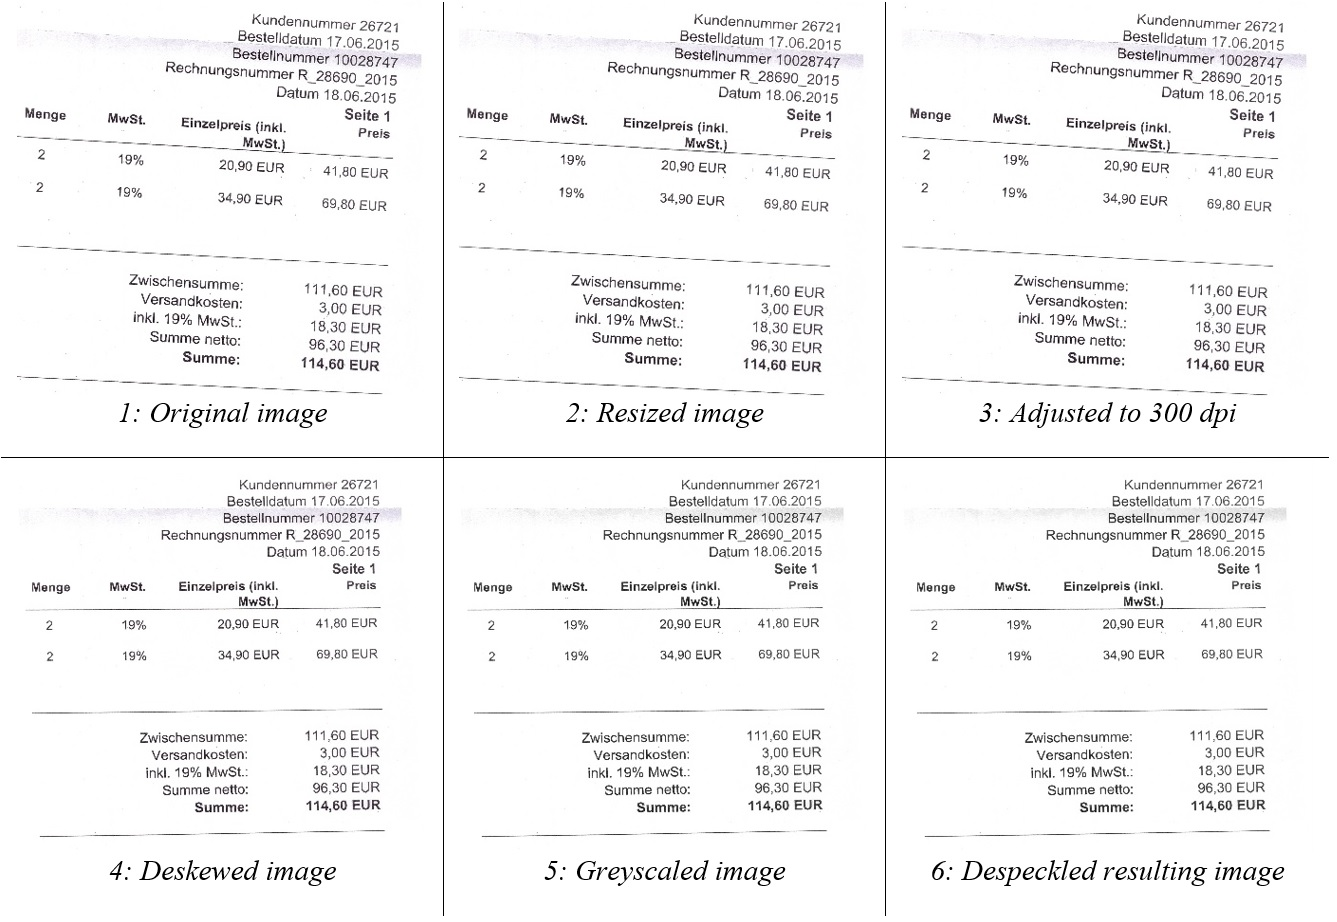
\includegraphics[width=\textwidth]{Images/OCR/PreprocessingSteps.jpg}
\caption{Preprocessing steps \label{preprocessingSteps}}
\end{figure}

The resulting changes in the image during the preprocessing steps are shown in figure \ref{preprocessingSteps}.
Especially the deskewing step and the greyscaling of the image can be seen very well.

In order to increase the performance of the application, we want to be able to perform the optical character recognition by using multiple instances of the tesseract at the same time. Hence we need to implement the Runnable interface provided by the JDK. 

Seen from the outside, the TesseractWrapper class is just the Tesseract instance itself. So we need a worker class that can be given to a new Thread. The TesseractWorker class implements this interface. When we start a new Thread using start(), the run()-method of this worker is called internally. Run initiates a new Tesseract instance and executes OCR with the given ocr file: 

\begin{lstlisting}[caption={Initiation of the OCR wrapper}]
/**
 * Executes tesseract ocr using a wrapper
 * The result can be obtained using the getResultIfFinished() method
 */
@Override
public void run() {
    TesseractWrapper wrapper = new TesseractWrapper();
    if (this.imgToScan == null) {
        this.result = wrapper.initOcr(this.fileToScan, runWithHocr);
    } else {
        this.result = wrapper.initOcr(this.imgToScan, runWithHocr);
    }
    Logger.getLogger(this.getClass()).log(Level.INFO, "Finished OCR");
}
\end{lstlisting}

Since we want to be able to support not only pdf documents, but also images, we have to differentiate between this two. Depending what type of document, we have to parse it differently in order to get a BufferedImage out of it.

After the OCR process took place, we have a HOCRDocument. It may be that some of the values are wrong, e.g. have a wrong but similar looking letter in it. This is not a problem as long as specific keywords are not affected. Recognizing such keywords in the document is crucial for the next steps. Hence we want to improve those values afterwards. 
The Postprocessor class targets this goal by going through the HOCRDocument:

\begin{lstlisting}[caption={Postprocessing the hocr document}]
        List<String> correctWords = this.readDictionaryValues();
        for (HocrPage page : this.documentToProcess.getPages()) {
            for (HocrElement area : page.getSubElements()) {
                for (HocrElement paragraph : area.getSubElements()) {
                    for (HocrElement line : paragraph.getSubElements()) {
                        for (int i = 0; i < line.getSubElements().size(); i++) {
                            HocrWord w = (HocrWord) line.getSubElements().get(i);
                            for (String dictWord : correctWords) {
                                // replace the word if the dictionary word is probably the right word
                                double confidenceRate = ConfigHelper.getConfidenceRate();
                                double distance = StringUtils.getLevenshteinDistance(w.getValue().toLowerCase().trim(), dictWord.toLowerCase().trim());
                                double comparison = distance / w.getValue().length();
                                if (comparison < confidenceRate) {
                                    w.setValue(dictWord);
                                    line.getSubElements().set(i, w);
                                    break;
                                }
                            }
                        }
                    }
                }
            }
        }
        return this.documentToProcess;
\end{lstlisting}

This is done using a dictionary of keywords. This dictionary is present as a file 'keywords.txt' and enables further improvements by the user (e.g. adding more keywords because of invoice documents in other languages).
The distance is calculated using the Levenshtein distance again. If the distance is small enough, the value of the HocrWord object is replaced by the keyword in the keywords.txt file.

Now that we have executed the OCR step and postprocessed the resulting values, the next module can go on in the complete process.

\section{Module 2 - Extraction}
\label{sec5.5}

The core class that extracts the information from the hocr document is the DataExtractorService class. As we also want to retrieve information as fast as possible, we want to run it on different threads, so that we can extract the invoice information part on one thread and the accounting records information on another. Hence this class needs to implement the Runnable interface. When instantiated, a flag is set if this thread should extract the former or the latter:

\begin{lstlisting}[caption={Beginning of the information extraction}]
@Override
public void run() {
    ...
    if (this.extractInvoice) {
        this.threadInvoice = this.extractInvoiceInformationFromHocr();
    } else {
        this.threadRecord = this.extractAccountingRecordInformation();
    }
}
\end{lstlisting}

We will now start explaining the extractInvoiceInformationFromHocr() method in detail before continuing with the explanation of the extractAccountingRecordInformatio() method.
As we built our invoice information extraction process on similar invoices of the same creditor, the extractInvoiceInformationFromHocr() method starts with a search for the creditor:

\begin{lstlisting}[caption={Call for creditor in the database}]
...
result.setCreditor(this.getLegalPersonFromDatabase(this.getHocrDoument(), true));
if (result.getCreditor() != null) {
    result = this.getCaseInformation(result);
} else {
    String invNo = this.findInvoiceNumber();
    result.setInvoiceNumber(invNo);
    result.setIssueDate(this.findIssueDate());
    result.setDebitor(this.getLegalPersonFromDatabase(this.getHocrDoument(), false));
}
...
\end{lstlisting}

If we are not able to find the creditor in the database (because there was no invoice of this creditor yet) we will continue by searching for necessary invoice information by hand. This will be covered after the case information retrieval.

If a creditor is found, we get the case information of the corresponding creditor. A DocumentCase consists of a creditor to which it belongs as well as a keyword which relates the DocumentCase to one of the following:
\begin{itemize}
	\item Document type: The DocumentCase contains information where to find a keyword that defines the document as an invoice, a proforma invoice or a credit note.
	\item Invoice number: The DocumentCase contains information where to find the corresponding invoice number of the invoice.
	\item Invoice date: The DocumentCase contains information where the invoice date is being placed on the document.
	\item Creditor: The DocumentCase contains information where the name of the creditor usually is. This is being used for new documents that are not classified yet in order to improve the recognition of creditors.
	\item Debitor: The DocumentCase contains information where the name of the debitor usually is.
\end{itemize}

Besides the keyword and the creditor, there is also the position stored where one of those keywords can be found, as well as the creation date of the DocumentCase, which is being used so that newer cases get a higher priority. This way we can react on changing designs for example when a company decides to restructure their invoice documents.

In addition to that, a case id clusters all DocumentCases that are created on one document. With five keywords at hand, a maximum of five DocumentCases should be related to one document.

A flag isCorrect is also existing but set to false in the beginning. After the user has reviewed missing information and wants to store the revised documents, the case is compared with the given information. If there are no changes, we expect the case to be correct. Hence at this time we set isCorrect to true.
The getCaseInformation() method first retrieves all cases from the found creditor. Then, it sorts them to the corresponding cases.

For each keyword the corresponding cases contain position information of older documents where the keyword has been found. With that position at hand, the current HOCR document is being searched for a value at that position. The method findInCase() deals with this process:

\begin{lstlisting}[caption={Search for information in the DocumentCase}]
private HocrElement findInCase(List<DocumentCase> cases) {
    for (DocumentCase docCase : cases) {
        if (docCase.getIsCorrect()) {
            String[] position = docCase.getPosition().split("\\+");
            // 0: startX, 1: startY, 2: endX, 3: endY
            int[] pos = new int[] {
				Integer.valueOf(position[0]), 
				Integer.valueOf(position[1]), 
				Integer.valueOf(position[2]), 
				Integer.valueOf(position[3])
			};

            HocrElement possibleArea = this.document.getPage(0).getByPosition(pos, 50);
            if (possibleArea != null) {
                HocrParagraph possibleParagraph = (HocrParagraph)  possibleArea.getByPosition(pos, 30);
                if (possibleParagraph != null) {
                    HocrLine possibleLine = (HocrLine) possibleParagraph.getByPosition(pos, 30);
                    if (possibleLine != null) {
                        HocrWord possibleWord = (HocrWord) possibleLine.getByPosition(pos, 10);
                        if (possibleWord != null) {
                            return possibleWord;
                        } else {
                            // refine to multiple words, pixel threshold only a few pixels since we are searching for word
                            possibleWord = possibleLine.getWordsByPosition(pos, 10);
                            return possibleWord;
                        }
                    }
                }
            }
        }
    }
    return null;
}
\end{lstlisting}

We are only using the cases that have the flag isCorrect set to true. Then we compare all HocrElements in the document with the stored position. But, as there could also be some small differences (e.g. because the scans are hand-made and the document has not been placed on the exact same position every time) we apply a threshold value. Every element that is more or less consistent with the given position will be returned. Eventually, we will a word that matches the position, or, if the position stored contained multiple words, a combination of words. Those are concatenated and returned. If any of those steps fail, the method will return null.

This is repeated for each keyword. A new DocumentCase is created and the position added. Every keyword that has not been found will result in missing DocumentCases. After that, the invoice filled with the retrieved information will be returned.

As mentioned before, if we are unable to find a creditor, then we proceed with the document manually. Which means we are looking for keywords such as ''Rechnungsnummer'' (invoice no.) or ''Rechnungsdatum'' (invoice date) which are usually followed by the corresponding value. This is a fallback practice and will yield more errors due to missing position information. An invoice object with the found values will be returned all the same.

The extractAccountingRecordInformation() method deals with the problem of information retrieval with a different approach: It uses the extracted table information if a table has been found (TODO: Include in text). If not, the HocrDocument is searched for keywords that are usually appear in invoice tables.

The detection of a table is done using another class, the HistogramMaker. A table usually contains black lines that structure the containing information. These lines can be detected by counting the amount of black pixels. Lines that contain such structures will result in a peak in the histogram. 

\begin{figure}[h]
\centering
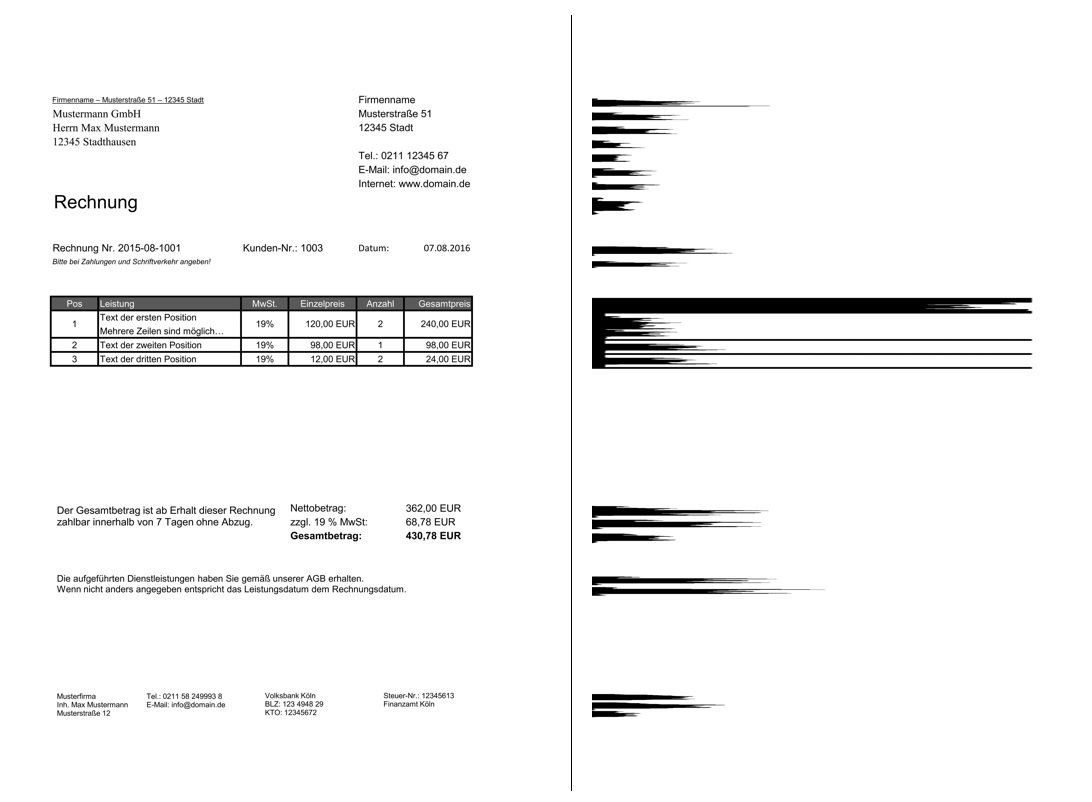
\includegraphics[scale=0.6]{Images/OCR/histogram.jpg}
\caption{Peaks of a table in the resulting histogram)  \label{histogramImage}}
\end{figure}

Figure \ref{histogramImage} shows a possible invoice document on the left side as well as the resulting histogram on the right. Note the peaks that indicate the tables in the invoice.

If we find those information, we iterate over the following lines until we find table end information, such as ''Gesamtbetrag'' (total value), ''Lieferdatum'' (delivery date) and others. Both, the table header words as well as table end words are stored in two textfiles (tablecontents.txt and tableendings.txt) which allows the user to add more words to improve the accuracy.
Now, every line will be processed the following way:

\begin{lstlisting}[caption={Manipulating and retrieving information from a position},label={arExtractionOne}]
Record r = new Record();
String recordLine = this.removeFinancialInformationFromRecordLine(nextLine);
double value = this.getValueFromLine(nextLine);
\end{lstlisting}

We first want to remove all those additional information from the position so that we are able to store / retrieve it if it comes again more precisely. This is done by the removeFinancialInformationFromRecordLine() method. After that, we also retrieve the total amount of the position by searching in the line again for the financial information, but this time searching for the last numeric value that is proceeded by ''EUR'' or ''\euro''. This behaviour is shown in listing \ref{arExtractionOne}.

\begin{lstlisting}[caption={Finding a model for the position},label={arExtractionTwo}]
Model m = service.getMostLikelyModel(recordLine); 
if (m == null) {
    r.setEntryText(nextLine);
} else {
    r.setEntryText(m.getPosition());
    r.setRecordAccounts(m.getAsAccountRecord(value));
    r.setProbability(m.getProbability());
}
records.add(r);
index++;
\end{lstlisting}

After that, the machine learning module is called. What exactly happens there will be covered by the next section. We will retrieve a possible Model that applies to our position. We can assign the found value to every involved account as the Model also contains the percentual values of each account and add a probability value to the Record which will later presented to the user in order to facilitate his decision if the automatically made decision is correct or not. This is shown in listing \ref{arExtractionTwo}.


\section{Module 3 - Machine Learning}
\label{sec5.6}

The Model object shown in listing \ref{arExtractionTwo} is a combination of debit and credit accounts (stored as a map with the corresponding values), the position string and the probability value. The LearningService class is the core class of this module and is getting called using the getMostLikelyModel() function. What this method does is the following:

\begin{lstlisting}[caption={Search for the most likely model}]
 public Model getMostLikelyModel(String feature) {
        String replacedString = feature;
        NaiveBayesHelper helper = new NaiveBayesHelper();
        ModelReader reader = new ModelReader();
        ...
            helper.trainClassifier(reader.getModels());

            // replace string if it is equal with an existing value
            for (Model m : reader.getModels()) {
                if (m.positionEqualsWith(feature)) {
                    replacedString = m.getPosition();
                    break;
                }
            }
		...
\end{lstlisting}

In the first part, the NaiveBayesHelper is called, that trains the classifier with all models that are stored. Every time the user saves an invoice document, all the accounting records are transformed into this model and saved to a file. The ModelReader takes these information for the next classification and hands it to the NaiveBayesHelper that is training the classifier.


To use the naive bayes classifier, we make use of a small implementation by Philipp Nolte, licensed under the MIT license\footnote{See also: https://github.com/ptnplanet/Java-Naive-Bayes-Classifier (Retrieved March 5, 2017)}.

When the classifier has been trained by the existing data, we compare the position with the ones stored in the existing models. This is done by a call to the model with positionEqualsWith(), that not simply compares the string, but also calculates the levenshtein distance. This is shown in listing \ref{positionComparison}.

\begin{lstlisting}[caption={Comparison between positions},label={positionComparison}]
    boolean positionEqualsWith(String positionToCompare) {
        int levDistance = StringUtils.getLevenshteinDistance(this.getPosition(), positionToCompare);
        int length = this.getPosition().length();
        double distance = (double) levDistance / (double) length;
        if (distance < 1 - ConfigHelper.getConfidenceRate()) {
            return true;
        } else {
            return false;
        }
    }
\end{lstlisting}

In the second part, the classifier is called and should now start classify the position. What this classifier does is basically the same as explained in section \ref{sec4.2.3}. The classification object also contains a probability value. We want this probability higher than a user set confidence rate in order to use the model.

If  this is the case, the ModelReader will be called again to retrieve the found model. This model will also be now be used in the transformation process 

\begin{lstlisting}[caption={Classification of a position}]
        Classification<String, List<Account>> classification = helper.getClassifier().classify(Collections.singleton(replacedString));
        if (classification.getProbability() > ConfigHelper.getConfidenceRate()) {
            try {
                Model m = reader.getModelByStringAndAccounts(String.valueOf(classification.getFeatureset().toArray()[0]), classification.getCategory());
                m.setProbability(classification.getProbability());
                return m;
            } catch (IOException e) {
                e.printStackTrace();
                return null;
            }
        }
        return null;
    }
\end{lstlisting}

However, if the probability is below the confidence rate, or any other problem might occur, null will be returned. This way only the position value will be set and the user has to manually check this accounting record (as can be seen in listing \ref{arExtractionTwo}).
    
\section{Module 4 - Transformation}
\label{sec5.7}

We have now extracted required basic information of the invoice as well as accounting records based on the positions in the invoice. Everything has been labelled by a confidence level in the application. All documents with a confidence level lower than previously defined by the user had to be reviewed by the user manually.
The final part of the use case is the transformation of those extracted information into the ZugFerd invoice format. Therefore, we need to order the given information in a predefined format and append it as xml-information to the invoice pdf.

We are using the Mustang project to generate the xml content for us. It is an open source project licensed under the Apache license version 2.0 and currently under version 1.3. This way, the amount of classes we need will be reduced to only one: The ZugFerdTransformator.java class.

Before giving an in-depth explanation about our implementation, we first want to explain how the ZugFerd-Format works.

\subsection{About the ZugFerd Scheme}
\label{sec5.7.1}

ZugFerd has been developed to close the gap between manually sent invoices in small companies and heavy electronic data interchange (EDI) between big companies. While EDI with its sub-standards can be a good solution for a big company, most of the small and medium sized companies can not make use of such a standard due to the overwhelming complexity that lies beyond this standard. But dealing with pdf documents manually is also a source of costs, errors and is time consuming. ZugFerd stands in the middle between those two sides (figure \ref{zugFerdImage} visualizes this).
\begin{figure}[htb!]
\centering
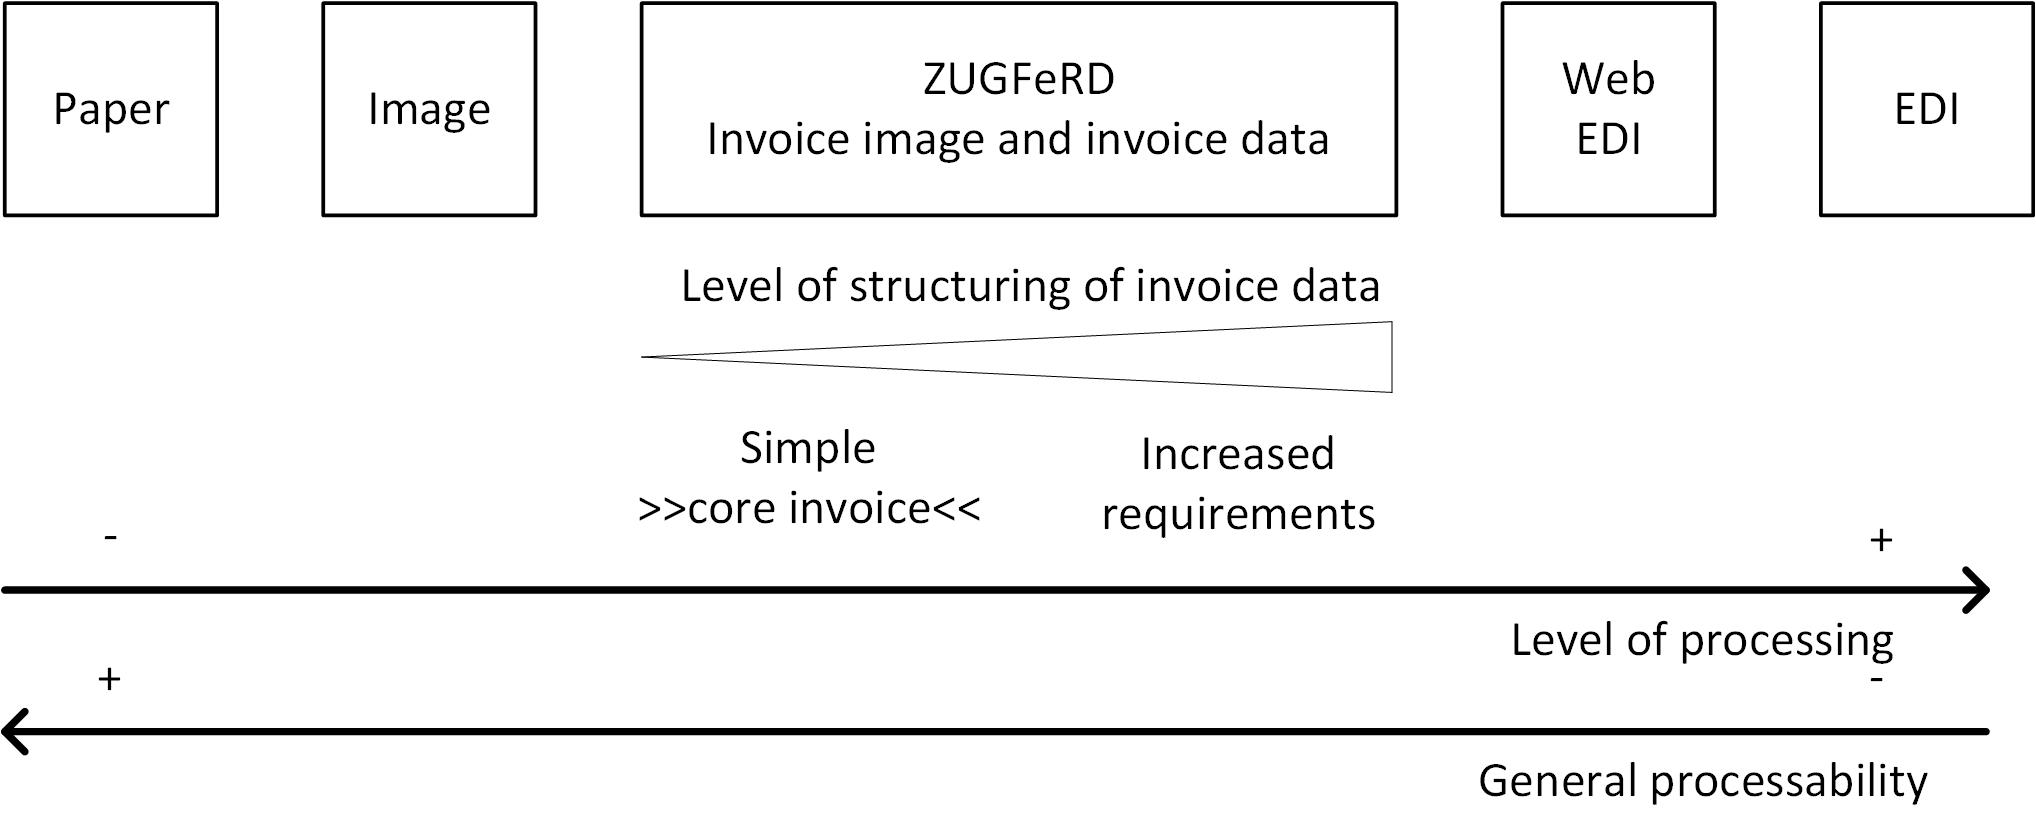
\includegraphics[width=\textwidth]{Images/ZugFerd/ZugFerd_English.jpg}
\caption{ZugFerd stands between paper invoice and edi-ready invoice (based on \cite[page 13]{zugFerdSpecificationEnglish})  \label{zugFerdImage}}
\end{figure}

While documents can still be sent as a pdf, the underlying format enables automatic processing of the invoice. The extendibility with basic, comfort and extended levels enables also big companies to make use of this standard. This also improves the B2B relations between big and small companies.

Depending on the desired level of the ZugFerd format, more fields have to be filled out. But even the lowest level, the basic level, brings the possibility to provide additional information which would only be required on the comfort or extended level. But there are still some fields that even on the basic level are required. Those will be introduced now and explained shortly.
\begin{itemize}
	\item Document Context Parameter: This field describes which level will be used in this document. A possible option would be the comfort-level.
	\item Exchanged Document Identifier: A unique identifier for an invoice. This is usually the invoice number that is present in the invoice document.
	\item Exchanged Document Type Code: The type code defines the invoice more in detail. There are currently three codes available: 380, 84 and 389.
	
In the basic level, only code 380 is supported. All invoices regarding goods or services, as well as credit notes and payment requests should be labelled with this code.
Beginning with the Comfort-level, code 84 is also supported. It refers to invoices without goods or values as well as credit notes without goods or values.
Only the Extended-level supports code 389, which is a special case for self-filled invoices or credit notes.
Exchanged Document Issue Date: The date when the invoice has been issued.
	\item Trade Agreement Seller Trade Party Name: The name of the company that is selling the goods or services in the invoice (also known as the creditor of the invoice).
	\item Trade Agreement Buyer Trade Party Name: The name of the company or person that bought the goods or services and to whom this invoice is addressed at (also known as the debitor of the invoice).
	\item Supply Chain Trade Settlement Invoice Currency Code: This field describes the kind of currency that is used in the invoice. Countries in the European Union and Germany in particular will mostly be using ''EUR'' as the Code for Euro currency, but there are also codes for US Dollar (''USD''), the Britain pound (''GBP'') and the Columbian peso (''COP'') available.
	\item Trade Settlement Monetary Summation Line Total: Line total is the total value of all positions combined.
	\item Trade Settlement Monetary Summation Charge Total: This field contains the sum of all additional charges to the invoice. These are not the price of the goods or services, but more additional costs (for instance: delivery costs, cancellation charges or reminder fees).
	\item Trade Settlement Monetary Summation Allowance Total: The sum of all allowances made on this invoice (e.g.: parts of the goods that are tax-free).
	\item Trade Settlement Monetary Summation Tax Basis Total: The net total on which the tax will be calculated.
	\item Trade Settlement Monetary Summation Tax Total: The total tax value that is applied on the invoice.
	\item Trade Settlement Monetary Summation Grand Total: The total sum of the invoice (usually the net total added by the tax that has been applied).
\end{itemize}

These are the most important fields in the ZugFerd format. Without them, it is not possible to create a conformal invoice document. This only applies on the Basic level of the ZugFerd format. Using the Comfort or even Extended-Level, several other fields are required. We will not further introduce these additional fields since the support of the other levels is not part of this thesis. 

\subsection{The transformation process}
\label{sec5.7.2}

We have now introduced all the necessary fields to create an invoice document which fulfils the requirements of the ZugFerd-Scheme Basic level and can now explain the actual transformation process. 

When the user decides to save the invoice, the DatabaseService is called. The saveProcessResult() method first saves the invoice object and then tries to save the scan object. Now, the ZugFerdTransformator class comes in place. The transformator object transforms the invoice to a ZugFerd invoice using the Mustang framework. This transformation will be explained shortly after. After the ZugFerd invoice has been appended to the document, a scan object is saved. This can be seen in listing \ref{saveScan}.

\begin{lstlisting}[caption={}, label={saveScan}]
        Invoice i = result.getExtractionModel().getUpdatedInvoiceInformation();
        ...
        Scan scan = new Scan();
        try {
            ZugFerdTransformator transformator = new ZugFerdTransformator();
            byte[] file = Files.toByteArray(result.getFile());
            byte[] enhancedFile = transformator.appendInvoiceToPDF(file, i);
            scan.setFile(enhancedFile);
            scan.setCreatedDate(Date.valueOf(LocalDate.now()));
            scan.setInvoiceInformation(i);
            ScanDao scanDao = new ScanDaoImpl();
            scanDao.save(scan);
        }
\end{lstlisting}

Let us have a detailed look on the ZugFerdTransformator.java class. The core method of this class is the createFullConformalBasicInvoice() method. 
In the first part, an invoice object is created and meta information are provided:

\begin{lstlisting}[caption={Creation of the invoice object}]
Invoice i = new Invoice(BASIC);

Context con = new Context(BASIC);
Profile guideline = new Profile(BASIC);
guideline.setVersion(ProfileVersion.V1P0);
con.setGuideline(guideline);
\end{lstlisting}

This information defines the invoice object to be of the Basic level (it has been described before as the Document Context Parameter). The ProfileVersion is currently 1.0 but could be increased when the ZugFerd format is further developed.
A header containing the basic information of the invoice is now instantiated:

\begin{lstlisting}[caption={Populating header information}]
Header h = new Header();
h.setName("RECHNUNG");
h.setInvoiceNumber(inv.getInvoiceNumber());
h.setCode(_380);
h.setIssued(new ZfDateDay(inv.getIssueDate().getTime()));
\end{lstlisting}

As the application only deals with Invoices, we can set the name to ''RECHNUNG'' (engl.: invoice). The invoice number has been extracted from the invoice object that has been given to the method.
Since this method creates an invoice object of the Basic level, the only applicable code for this level is 380. Afterwards, the issue date of the given invoice object is used as well.

It is now time to add the actual invoice content. First, we have to define the creditor and debitor of this - in the terminology of the ZugFerd documentation - agreement. Both, the creditor and the debitor, are a TradeParty that are added to the agreement:

\begin{lstlisting}[caption={Creation of a new agreement}]
Agreement a = new Agreement();
a.setBuyer(new TradeParty().setName(inv.getDebitor().toString()));
a.setSeller(new TradeParty().setName(inv.getCreditor().toString()));
\end{lstlisting}

Hence we create a new Agreement object and set Buyer and Seller instances (respectively debitor and creditor) by using the given name of the legal person in the provided invoice object.

All the financial information such as Line Total or Tax Basis Total are now filled in to the MonetarySummation object:

\begin{lstlisting}[caption={Population of the MonetarySummation object}]
MonetarySummation sum = new MonetarySummation();
sum.setLineTotal(new Amount(BigDecimal.valueOf(inv.getLineTotal()), EUR));
sum.setChargeTotal(new Amount(BigDecimal.valueOf(inv.getChargeTotal()), EUR));
sum.setAllowanceTotal(new Amount(BigDecimal.valueOf(inv.getAllowanceTotal()), EUR));
sum.setTaxBasisTotal(new Amount(BigDecimal.valueOf(inv.getTaxBasisTotal()), EUR));
sum.setTaxTotal(new Amount(BigDecimal.valueOf(inv.getTaxTotal()), EUR));
sum.setGrandTotal(new Amount(BigDecimal.valueOf(inv.getGrandTotal()), EUR));

Settlement s = new Settlement();
s.setCurrency(EUR);
s.setMonetarySummation(sum);
\end{lstlisting}

The Settlement object holds this information. For each value, we also have to provide currency information. The application currently only supports invoices with the currency Euro, hence every amount will be added as the currency Euro.

To conclude the trade, we also have to define a delivery date. If no such information has been found in the invoice document, we will use the issue date as a fallback value:

\begin{lstlisting}[caption={Population of the trade object}]
Delivery d;
if (inv.getDeliveryDate() == null) {
    d = new Delivery(new ZfDateDay(inv.getIssueDate().getTime()));
} else {
    d = new Delivery(new ZfDateDay(inv.getDeliveryDate().getTime()));
}

Trade tr = new Trade();
Item item = new Item();
tr.addItem(item);
tr.setAgreement(a);
tr.setDelivery(d);
tr.setSettlement(s);
\end{lstlisting}

After that, a Trade object is being instantiated and the information are added. Note that we create an empty Item object for the trade. This is necessary for the invoice object to be valid. But only in the higher levels actual information regarding specific items are required to be provided.

Eventually, we add the context, the header information as well as the trade object to the actual invoice object:

\begin{lstlisting}[caption={Population of the invoice object}]
i.setContext(con);
i.setHeader(h);
i.setTrade(tr);
\end{lstlisting}

Before we now return the invoice document, we have to make sure that this document is valid against the ZugFerd-Scheme. Only if this invoice is valid, it will be returned, otherwise the method will return null:

\begin{lstlisting}[caption={Validation of the invoice object}]
if (this.isInvoiceValid(i)) {
    return i;
} else {
    return null;
}
\end{lstlisting}

The isInvoiceValid() method makes use of an InvoiceValidator, which is given by the Mustang framework and enables us to quickly validate the invoice object:

\begin{lstlisting}[caption={Usage of the InvoiceValidator object}]
InvoiceValidator invoiceValidator = new InvoiceValidator();

Set<ConstraintViolation<Invoice>> violations = invoiceValidator.validate(i);
return violations.size() < 1;
\end{lstlisting}

The InvoiceValidator does not only check if the required fields are filled out, but also makes calculations on the MonetarySummation object. For instance, if the provided tax value does not sum up correctly to the grand total or the tax basis is smaller than the actual tax (which would mean a tax value over 100\%) an error will be raised.
With the correct validation of the invoice object the task of this module is completed. 

\section{Module 5 - GUI}
\label{sec5.8}
The complete application is also supported by a graphical user interface which facilitates working with it.
As defined in section \ref{sec5.2} before, we will not only enable the user to extract information, but also retrieve stored invoices later on. This section will first go through the process of invoice information extraction and deal with invoice retrieval later on. In the end, a settings site will presented and explained as well.

\subsection{Scanning and reviewing an invoice document}
\label{sec5.8.1}

When starting the application, a startpage opens. As the first process of the application would be the scanning of a document, a button already hints to the task of scanning a form. This can be seen in figure \ref{startmenu}.
\begin{figure}[ht!]
\centering
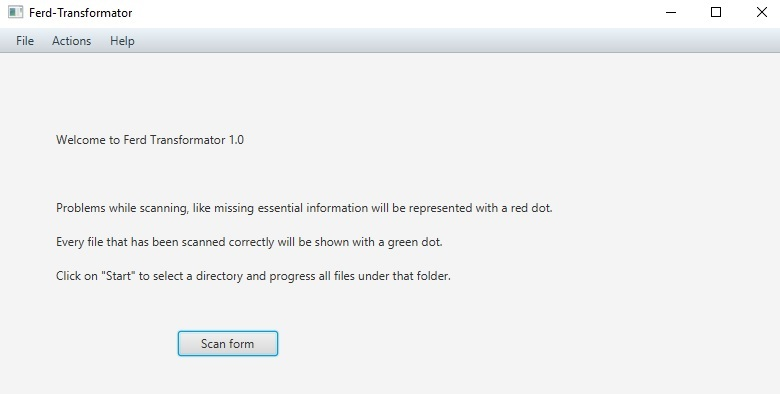
\includegraphics[scale=0.6]{Images/GUI/startmenu.jpg}
\caption{The start page of the application \label{startmenu}}
\end{figure}

In the top there are the menus \emph{File}, \emph{Actions} and \emph{Help}. The \emph{File} menu provides the settings (as discussed in \ref{sec5.7.3}) and the close application actions.
\emph{Actions} also contains the possibility of starting to process a form directory, as well as the search function (as explained in \ref{sec5.7.2}.
\emph{Help} contains information about the application (such as version, used frameworks etc.) and links to a help document.

After the user clicked on the 'Scan form' button, a file chooser opens where the user can choose a directory where the files are. When the user has selected a directory, the application begins processing the forms under that directory.

This process can be seen in figure \ref{processingFiles}.

\begin{figure}[ht!]
\centering
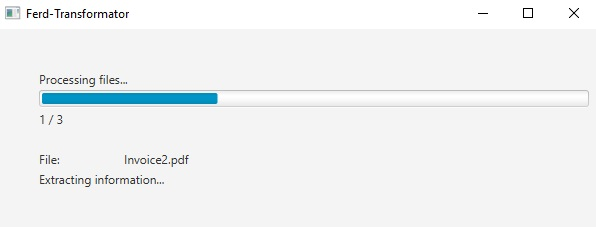
\includegraphics[scale=0.6]{Images/GUI/processingFiles.jpg}
\caption{Processing document files \label{processingFiles}}
\end{figure}

During the extraction process, a progress bar indicates the progress of the processing of the documents. In addition to that, the current file, the file name as well as the current state is provided to give the user a possibility to estimate the remaining time.

When the process has finished and all invoice documents have been processed, a new page opens. Instead of saving all documents automatically, this way the user has the possibility to revise the documents before.
The page with the table of all revised documents is shown in figure \ref{reviseBeforeSafe}.

\begin{figure}[ht!]
\centering
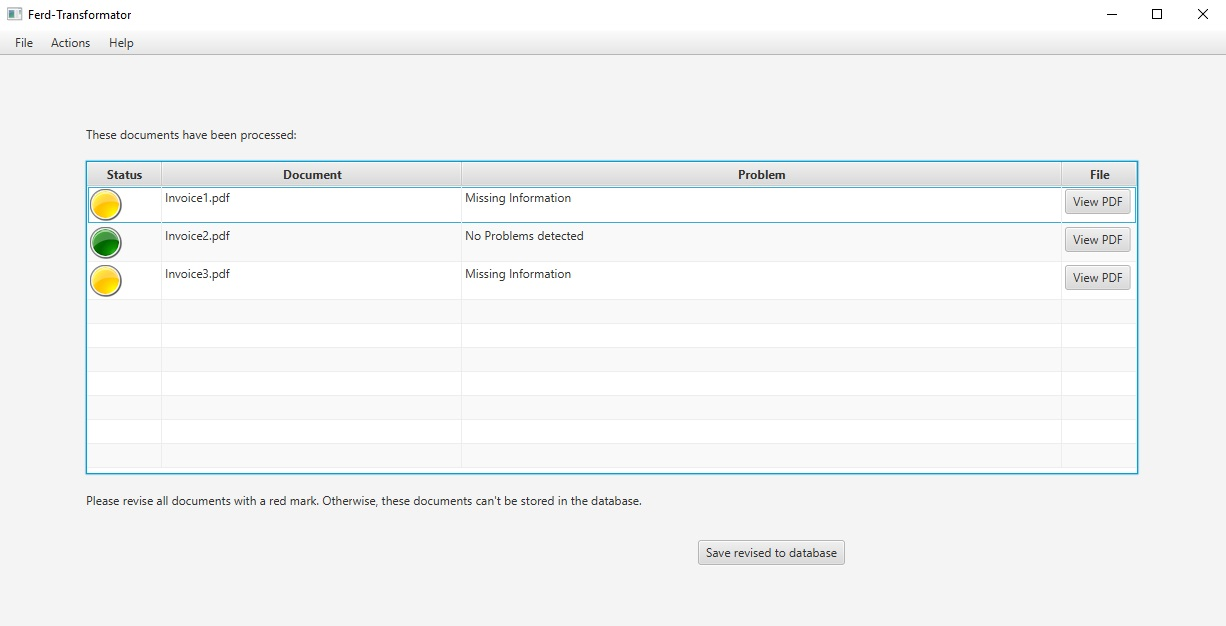
\includegraphics[width=\textwidth]{Images/GUI/reviseBeforeSafe.jpg}
\caption{Table with processed documents \label{reviseBeforeSafe}}
\end{figure}

In the first column, a coloured dots indicates possible problems with the documents. If there is a critical error in the code making it impossible to further process the document, the dot will be red. 
A yellow dot instead marks that the document has been processed successfully, but there are still issues with the documents which make it not possible to save the document at this time.
If the dot is green, these documents can instantly be saved to the database. If in doubt, the user can still access those documents too in order to check the values.

The second column contains the document name. In the third column possible problems are listed. This way the user can find out specific problems more easily.

The last column contains a button which allows the user to access the detail view of this document. There are two detail pages per document: One for basic invoice information and one for the accounting record positions.

Figure \ref{reviewElectronicInvoice} shows the first detail view.

\begin{figure}[htb!]
\centering
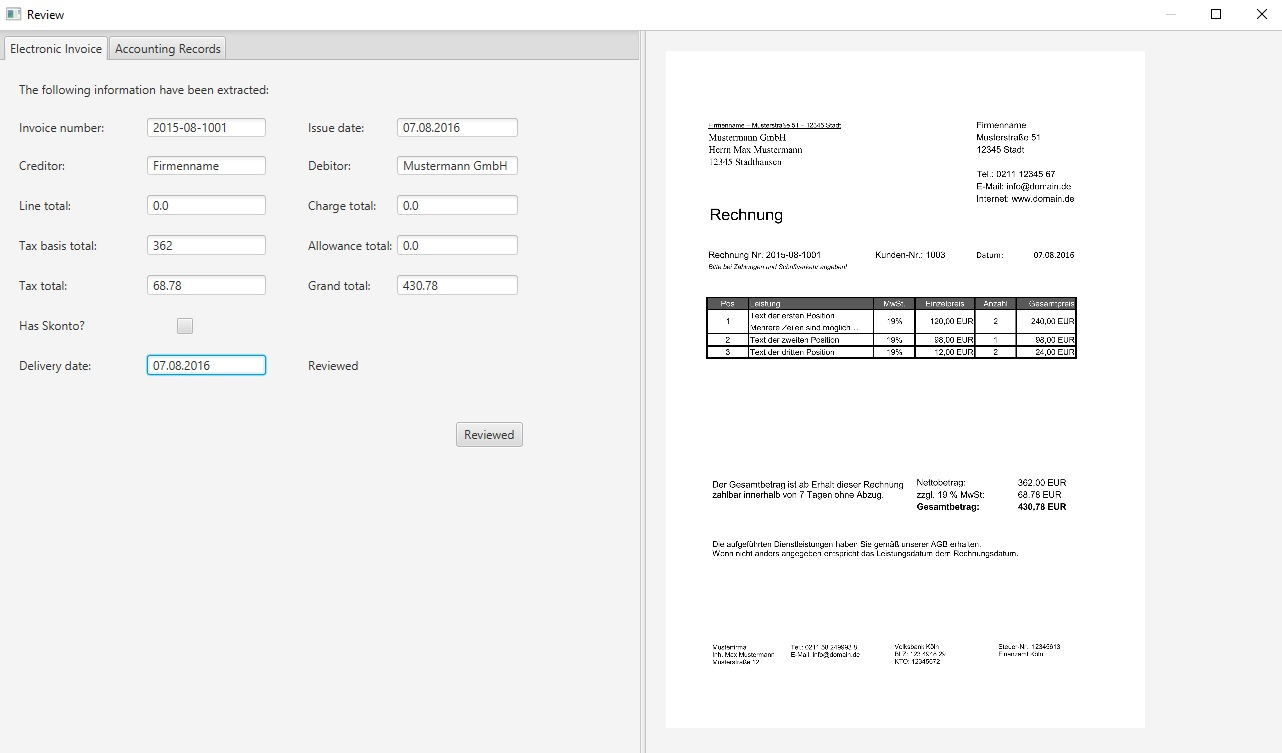
\includegraphics[width=\textwidth]{Images/GUI/ReviewElectronicInvoice.jpg}
\caption{Detail view of invoice information \label{reviewElectronicInvoice}}
\end{figure}

On the left side all the necessary information are present, while on the right side the invoice document can be seen. The user has the possibility to move the document around and zoom in and out. This is useful, if there are missing information that the user has to add in the case of missing information.

The required information on the left side are the ones required for a full conformal ZugFerd invoice of BASIC level. The amount of input fields could be enhanced in the future in order to support the COMFORT or even EXTENDED level.

All the values that have been extracted are set in to these fields. If the application was unable to extract information regarding a specific field, it will be left blank. If the user fills out the missing fields and forgets one, a validation message will be shown up, making it impossible to safe the document before filling out all fields.

If there is a Skonto applicable to the invoice, checking the checkbox 'Has Skonto?' will reveal another input field where the user is asked to provide the skonto value.

On the top left side of the image, there is also the possibility to switch between the general invoice information and the accounting records information. These information are shown in figure \ref{reviewAR}.

\begin{figure}[ht!]
\centering
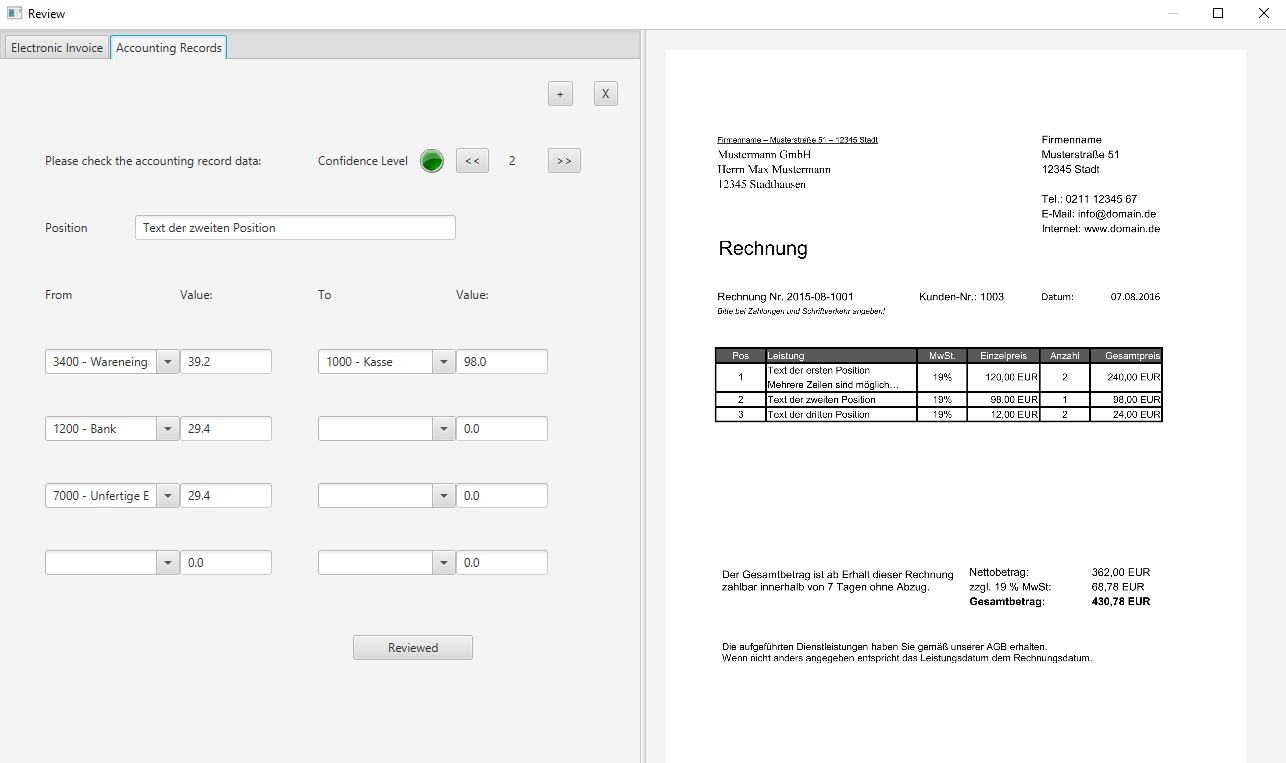
\includegraphics[width=\textwidth]{Images/GUI/ReviewAR.jpg}
\caption{Detail view of accounting record information \label{reviewAR}}
\end{figure}

This detail view looks slightly different. Positions that have been found by the application are written in the position field. But, as there can be more than position, there is the option to switch between each accounting record with the buttons in the top right of this part of the view.

For each position, there is the possibility to assign up to 8 accounts that can be involved in the accounting process (4 debit and 4 credit accounts). The amount of accounts is limited to 8, but could be enhanced in the future if there is a real need for it.

Each field of accounts can be searched for a specific name or account number, which makes working with all these accounts easier.

Note that there is a coloured dot next to the button to switch between accounting records. This dot is also an indicator how plausible the assignment is. 

In the top right corner of this side of the view there is also a '+' and a 'x' button. These can be used to add or remove accounting records as required by the user.

If the user hits the 'reviewed' button both, the invoice information as well as the accounting record information are validated. This includes:
\begin{itemize}
	\item Checking for all fields if a value is present.
	\item Calculating the values in the invoice information tab: The tax basis added by the tax total should equal the grand total value.
	\item Validating for each accounting record that:
		\begin{enumerate}
			\item There is at least one account on both, the credit and debit side
			\item An account is only used once
			\item The sum of the values of the credit side equals the sum of the values of the debit side
		\end{enumerate}
	\item Checking for empty accounts where a value has been written in
\end{itemize}

If any of these checks fail, a popup will show up and provide information which specific issues are persistent. The document can not be saved in this case. If there are no validation errors, the values are updated, the detail view closes and the user is returned to the list of the documents.

Note that the dot of the manually reviewed document has now changed from yellow to green (figure: \ref{greenAfterReview}) indicating that this document can now be saved.

\begin{figure}[ht!]
\centering
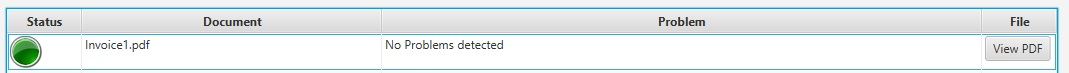
\includegraphics[scale=0.6]{Images/GUI/GreenAfterReview.jpg}
\caption{Changing of the dot after manually reviewing the document \label{greenAfterReview}}
\end{figure}

When the user eventually clicks on 'Save revised to database', all documents with a green dot will be saved. This will also be indicated by the application with a short popup which can be seen in figure \ref{savingSuccessful}.

\begin{figure}[ht!]
\centering
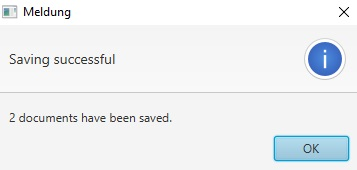
\includegraphics[scale=0.6]{Images/GUI/SavingSuccessful.jpg}
\caption{A popup that indicates the successful saving of the documents \label{savingSuccessful}}
\end{figure}

After the saving of the document, this process is completed. The user has now the possibility to navigate over 'Actions' and either scan other documents or retrieve documents from the database. This will be covered now in the following section.

\subsection{Searching for documents in the database}
\label{sec5.8.2}

After the processing of the document, the user very likely wants to retrieve the converted document. But also older documents that once have been processed should be retrievable again.
Figure \ref{searchInDatabase} shows the possible input information. 

\begin{figure}[ht!]
\centering
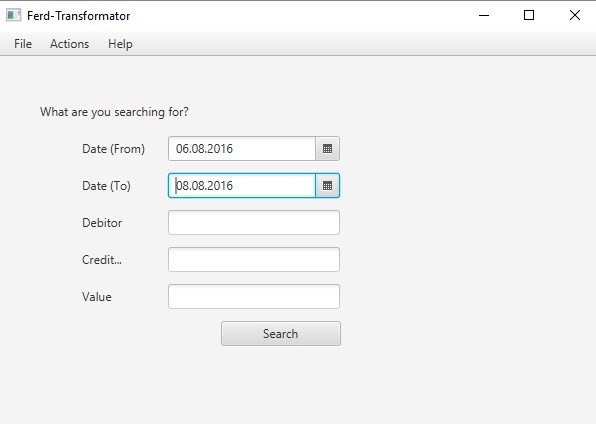
\includegraphics[scale=0.6]{Images/GUI/SearchInDatabase.jpg}
\caption{Possible search filters for stored documents \label{searchInDatabase}}
\end{figure}

The user is able to search for invoices either on a specific date (by leaving the 'date (from)' field blank) or a timespan.
It is also possible to search for a specific creditor or debitor name or a specific value of the invoice.
None of these fields have to be filled out. It only narrows the search as a filter and will facilitate the process of retrieving the desired invoice document.

As there is always the possibility that a user is trying to inject malicious code, the application is programmed with parameterized queries to prevent such possible SQL injections.

When the values have been set and the user has clicked on the button 'Search in database' a list of stored invoice documents that match the filter criteria is shown (figure \ref{searchResults}).

\begin{figure}[ht!]
\centering
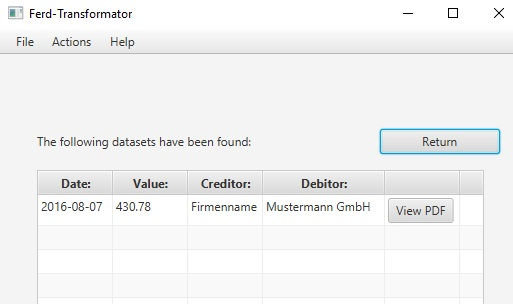
\includegraphics[scale=0.6]{Images/GUI/SearchResults.jpg}
\caption{The results of the database search \label{searchResults}}
\end{figure}

In this list, the existing information are shown to facilitate the finding of a specific invoice. By pressing the button 'View PDF' the user is able to save the file and view it. This invoice file also contains the added electronic invoice information of the ZugFerd standard.

Pressing 'Return' enables the user to re-enter search criteria. 

\subsection{Additional settings}
\label{sec5.8.3}

To make the application flexible and adjustable to the needs of the user, we provide several possible configuration settings that can be adjusted in the settings view. This view contains of four tabs, each of them deals with settings to a specific part of the application.
Figure \ref{settings_General} shows the general settings tab. 

\begin{figure}[ht!]
\centering
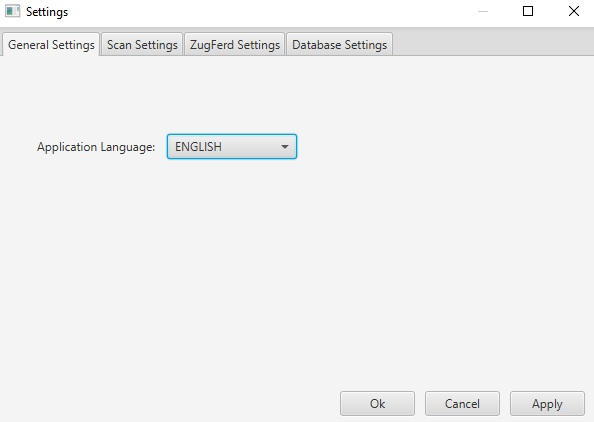
\includegraphics[scale=0.6]{Images/GUI/settings_General.jpg}
\caption{General settings tab \label{settings_General}}
\end{figure}

This tab only contains the overall language of the application at the moment. More general settings could be added in the future. By selecting German as the application language the whole GUI will change its appeareance.

\begin{figure}[ht!]
\centering
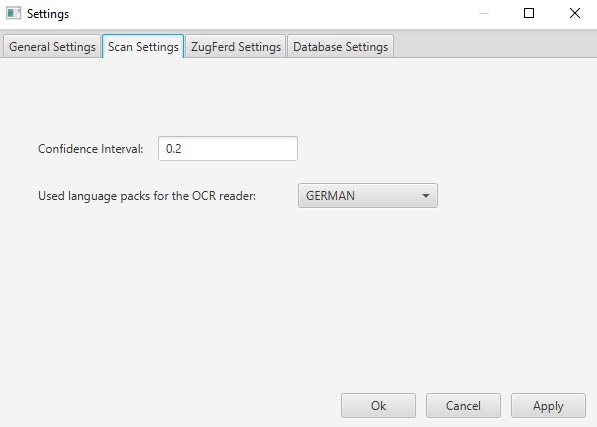
\includegraphics[scale=0.6]{Images/GUI/settings_Scan.jpg}
\caption{Scan settings tab \label{settings_Scan}}
\end{figure}

The scan tab shows two possible options: The confidence interval and the used language packs for the OCR reader. The former value has a significant influence not only to the evaluation of the Levenshtein-Distance, but also regarding the confidence of the accounting records (which is represented as a coloured dot). A value of 0.2 means a maximum difference of 20\% or in other words: A confidence level of 80\%.

The language packs for the OCR reader are important to increase the overall OCR accuracy. If the user only uses German invoices with German words in it, the German package enables the best accuracy. But if there are other keywords or English words in general that appear in some invoices, the combination 'English and German' would deliver the best results. Pure english invoices can also be processed using the 'English' language pack.

\begin{figure}[ht!]
\centering
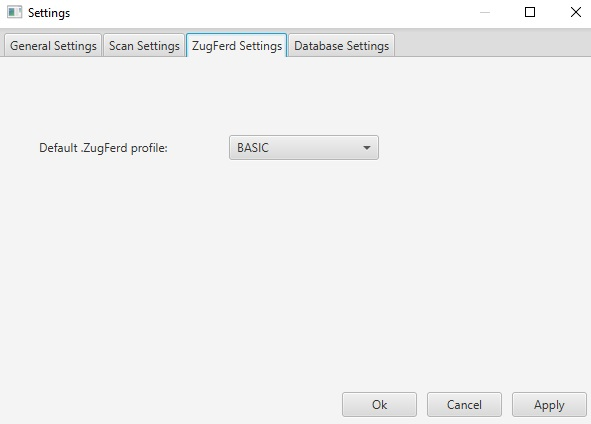
\includegraphics[scale=0.6]{Images/GUI/settings_ZugFerd.jpg}
\caption{ZugFerd specific settings tab \label{settings_ZugFerd}}
\end{figure}

The ZugFerd tab enables the user to choose between a preferred ZugFerd level (figure \ref{settings_ZugFerd}). As of now, the application only supports the BASIC level. When the application supports Comfort or Extended level in the future, this setting would enable a different view in the invoice information detail view.

\begin{figure}[ht!]
\centering
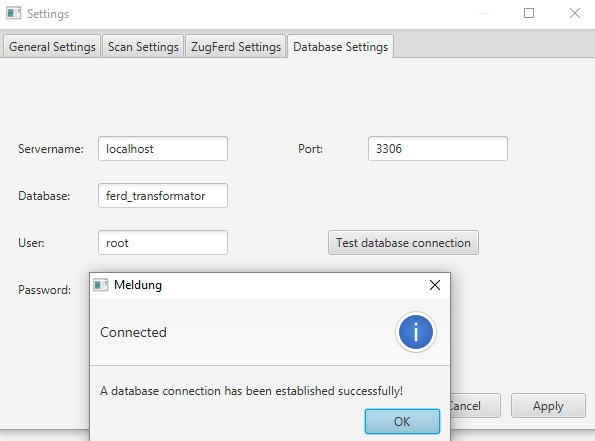
\includegraphics[scale=0.6]{Images/GUI/settings_Database.jpg}
\caption{Database connection settings tab \label{settings_Database}}
\end{figure}

The last tab, database settings, contains several database values that can be set to a specific database. The button 'Test Connection' enables a quick connection check and returns a popup with information if the connection was successful (see also figure \ref{settings_Database}). 